% This is a template file for Sweave used in MAGeCK
% Author: Wei Li, Shirley Liu lab
% Do not modify lines beginning with "#__".
\documentclass{article}

\usepackage{amsmath}
\usepackage{amscd}
\usepackage[tableposition=top]{caption}
\usepackage{ifthen}
\usepackage{fullpage}
\usepackage[utf8]{inputenc}
% \usepackage{longtable}

\usepackage{Sweave}
\begin{document}
\setkeys{Gin}{width=0.9\textwidth}

\title{MAGeCK Count Report}
\author{Wei Li}

\maketitle


\tableofcontents

\section{Summary}

%Function definition

%__FILE_SUMMARY__

The statistics of comparisons are listed in Table 1 and Table 2.
The corresponding fastq files in each row are listed in Table 3.

% latex table generated in R 3.6.3 by xtable 1.8-4 package
% Thu Apr  9 17:38:35 2020
\begin{table}[ht]
\centering
\begin{tabular}{ccccc}
  \hline
 & Label & Reads & Mapped & Percentage \\ 
  \hline
1 & baseline\_1 & 99687416 & 88216257 & 0.88 \\ 
  2 & fxn\_1 & 83380298 & 73132444 & 0.88 \\ 
  3 & baseline\_2 & 161628531 & 142728229 & 0.88 \\ 
  4 & fxn\_2 & 116718266 & 102431968 & 0.88 \\ 
   \hline
\end{tabular}
\caption{Summary of comparisons} 
\label{tab:one}
\end{table}
% latex table generated in R 3.6.3 by xtable 1.8-4 package
% Thu Apr  9 17:38:35 2020
\begin{table}[ht]
\centering
\begin{tabular}{ccccc}
  \hline
 & Label & TotalsgRNA & ZeroCounts & GiniIndex \\ 
  \hline
1 & baseline\_1 & 77736 & 43 & 0.07 \\ 
  2 & fxn\_1 & 77736 & 198 & 0.07 \\ 
  3 & baseline\_2 & 77736 & 75 & 0.09 \\ 
  4 & fxn\_2 & 77736 & 235 & 0.08 \\ 
   \hline
\end{tabular}
\caption{Summary of comparisons} 
\label{tab:two}
\end{table}




% latex table generated in R 3.6.3 by xtable 1.8-4 package
% Thu Apr  9 17:38:35 2020
\begin{table}[ht]
\centering
\begin{tabular}{cp{9cm}c}
  \hline
 & File & Label \\ 
  \hline
1 & 5\_Undetermined\_S0\_L001\_R1\_001\_TCGCAT.fastq & baseline\_1 \\ 
  2 & 6\_Undetermined\_S0\_L001\_R1\_001\_CATAGC.fastq & fxn\_1 \\ 
  3 & 8\_Undetermined\_S0\_L001\_R1\_001\_GTAGGC.fastq & baseline\_2 \\ 
  4 & 9\_Undetermined\_S0\_L001\_R1\_001\_TTCAAG.fastq & fxn\_2 \\ 
   \hline
\end{tabular}
\caption{Summary of samples} 
\label{tab:three}
\end{table}



The meanings of the columns are as follows.

\begin{itemize}
\item \textbf{Row}: The row number in the table;
\item \textbf{File}: The filename of fastq file;
\item \textbf{Label}: Assigned label;
\item \textbf{Reads}: The total read count in the fastq file;
\item \textbf{Mapped}: Reads that can be mapped to gRNA library;
\item \textbf{Percentage}: The percentage of mapped reads;
\item \textbf{TotalsgRNAs}: The number of sgRNAs in the library; 
\item \textbf{ZeroCounts}: The number of sgRNA with 0 read counts;
\item \textbf{GiniIndex}: The Gini Index of the read count distribution. Gini index can be used to measure the evenness of the read counts, and a smaller value means a more even distribution of the read counts.
\end{itemize}



\newpage\section{Normalized read count distribution of all samples}
The following figure shows the distribution of median-normalized read counts in all samples.


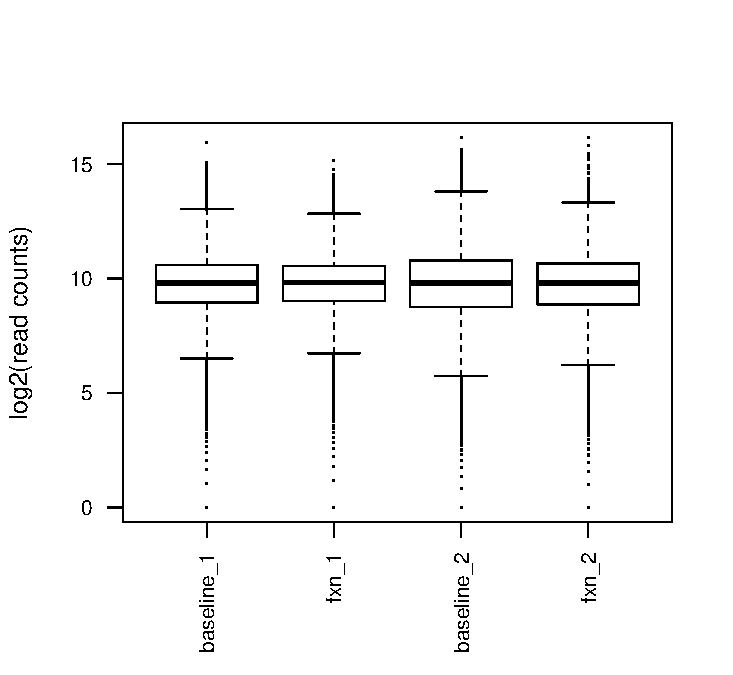
\includegraphics{count_20200409__countsummary-005}

The following figure shows the histogram of median-normalized read counts in all samples.


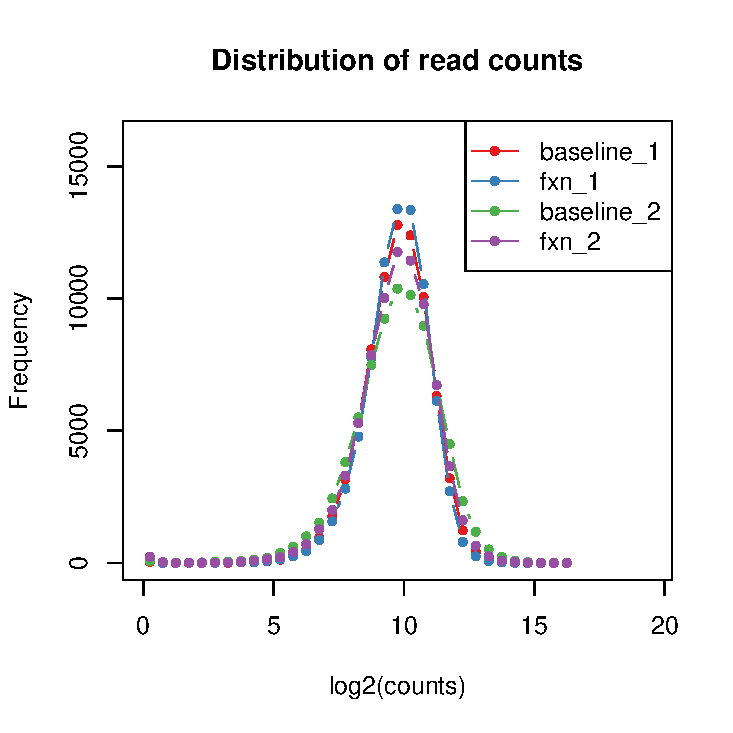
\includegraphics{count_20200409__countsummary-006}


\newpage\section{Principle Component Analysis}
The following figure shows the first 2 principle components (PCs) from the Principle Component Analysis (PCA), and the percentage of variances explained by the top PCs.



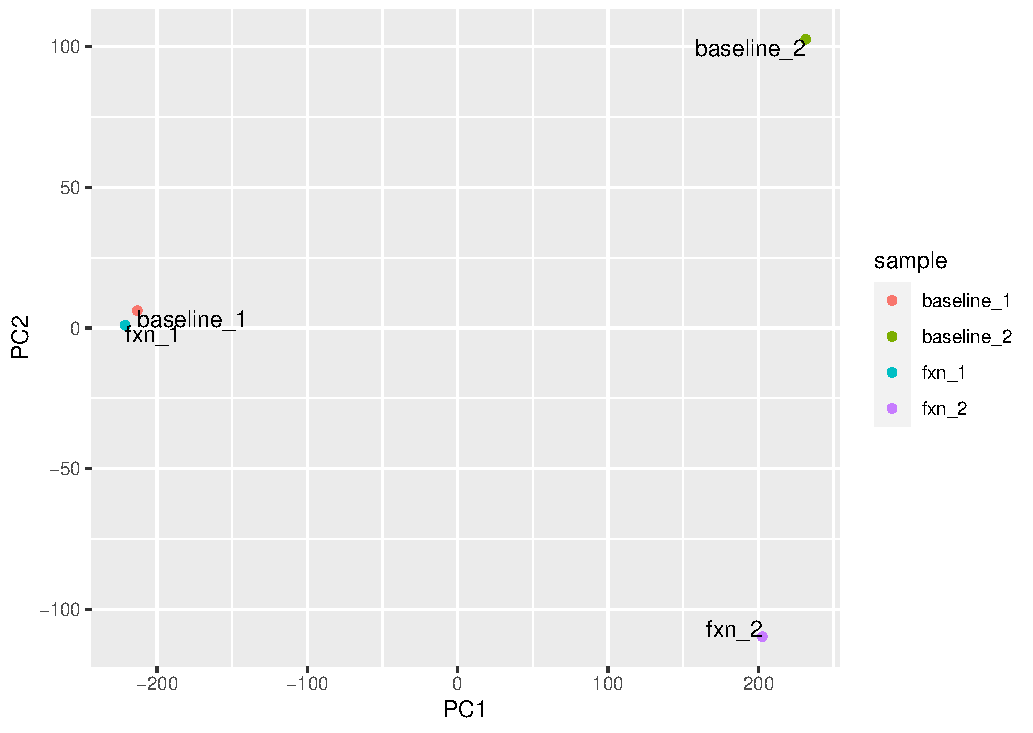
\includegraphics{count_20200409__countsummary-007}

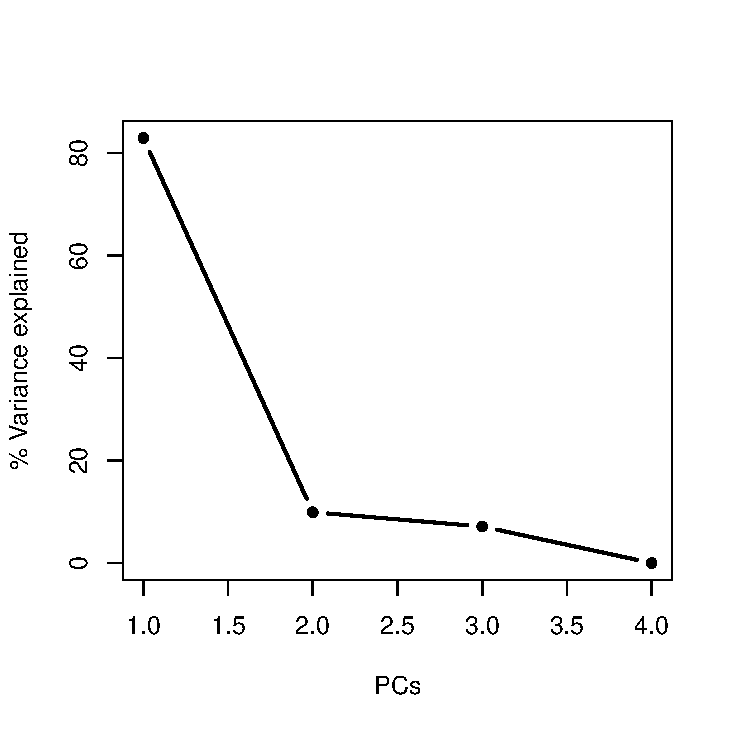
\includegraphics{count_20200409__countsummary-008}


\newpage\section{Sample clustering}
The following figure shows the sample clustering result.


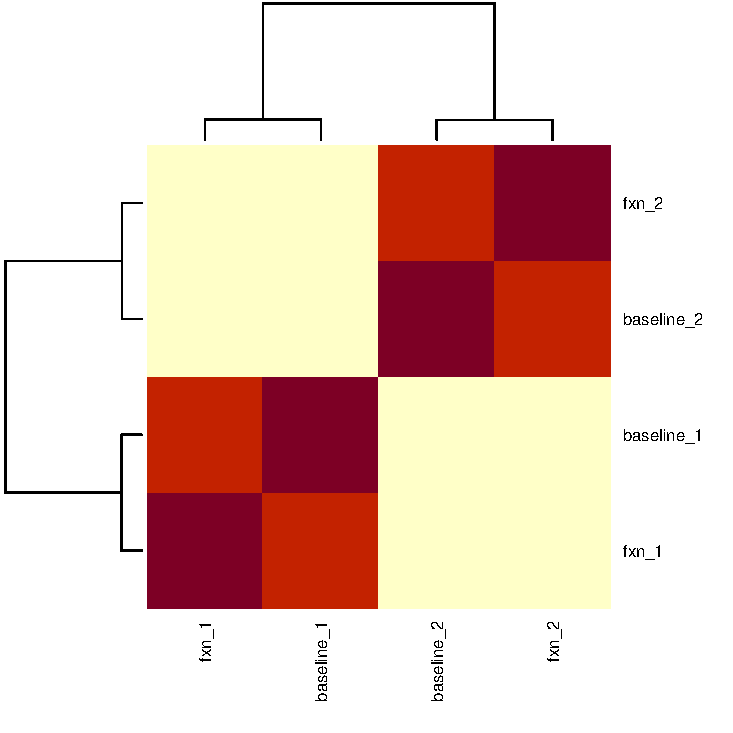
\includegraphics{count_20200409__countsummary-009}

%__INDIVIDUAL_PAGE__





\end{document}

